\documentclass{standalone}
\usepackage{tikz}
\usetikzlibrary{patterns, positioning}
\usepackage[sfdefault]{ClearSans} %% option 'sfdefault' activates Clear Sans as the default text font
\usepackage[T1]{fontenc}

\begin{document}
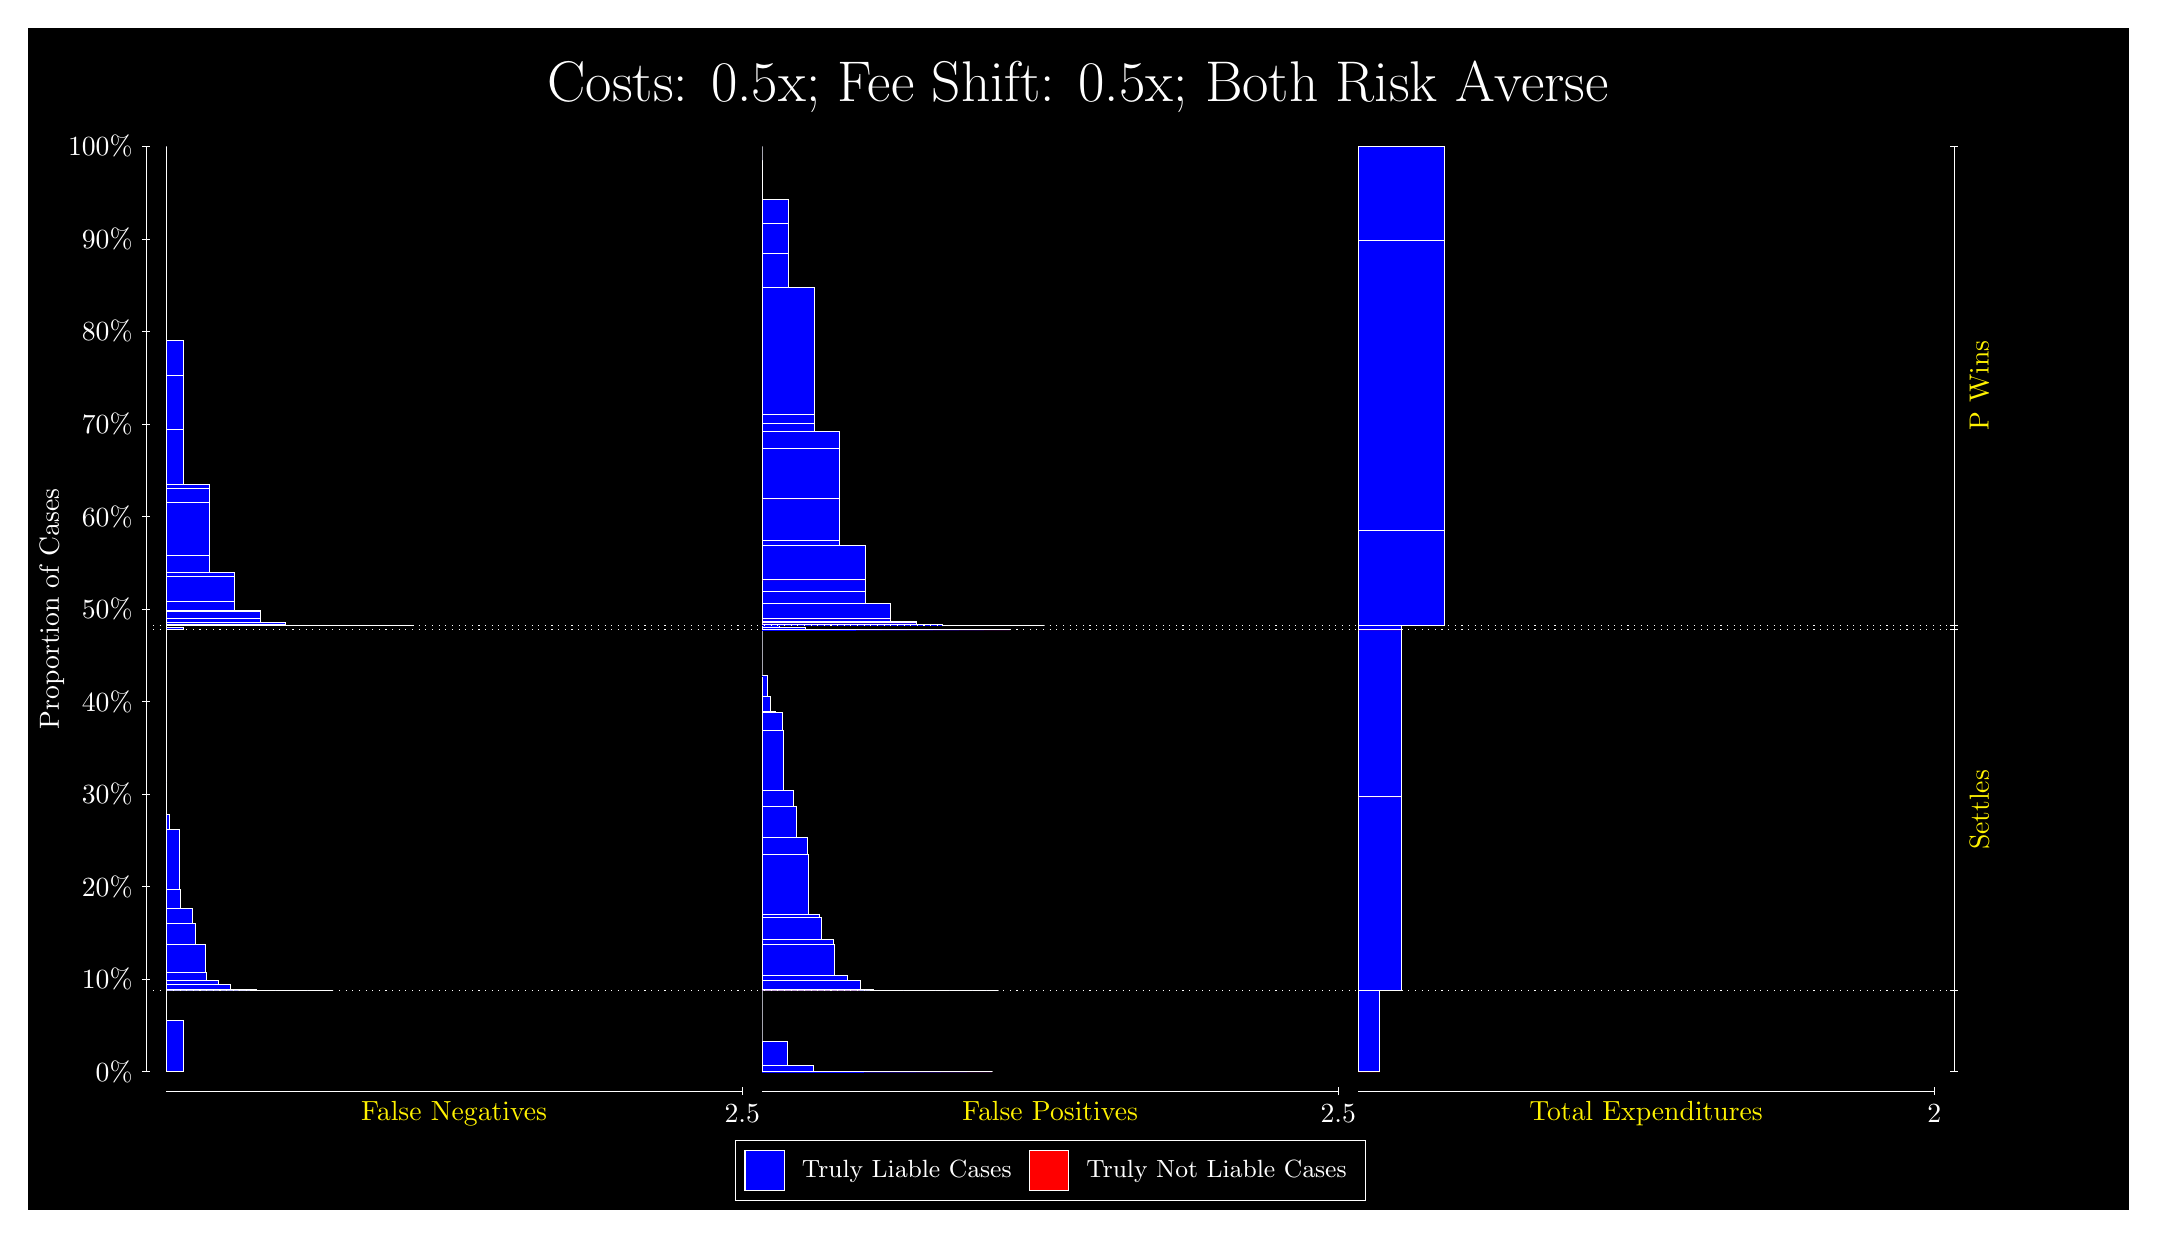
\begin{tikzpicture}
\draw[fill=black] (0,0) rectangle (26.667,15);
\draw[text=white] (0,13.5) rectangle (26.667,15) node[midway] {\huge Costs: 0.5x; Fee Shift: 0.5x; Both Risk Averse};
\draw[white, very thin] (1.5,1.75) -- (1.5,13.5);
\node[rotate=90, text=white, anchor=center] at (0.3, 7.625) {Proportion of Cases};
\draw[white, very thin] (1.45,1.75) -- (1.55,1.75);
\node[text=white, anchor=east] at (1.45, 1.75) {0\%};
\draw[white, very thin] (1.45,2.925) -- (1.55,2.925);
\node[text=white, anchor=east] at (1.45, 2.925) {10\%};
\draw[white, very thin] (1.45,4.1) -- (1.55,4.1);
\node[text=white, anchor=east] at (1.45, 4.1) {20\%};
\draw[white, very thin] (1.45,5.275) -- (1.55,5.275);
\node[text=white, anchor=east] at (1.45, 5.275) {30\%};
\draw[white, very thin] (1.45,6.45) -- (1.55,6.45);
\node[text=white, anchor=east] at (1.45, 6.45) {40\%};
\draw[white, very thin] (1.45,7.625) -- (1.55,7.625);
\node[text=white, anchor=east] at (1.45, 7.625) {50\%};
\draw[white, very thin] (1.45,8.8) -- (1.55,8.8);
\node[text=white, anchor=east] at (1.45, 8.8) {60\%};
\draw[white, very thin] (1.45,9.975) -- (1.55,9.975);
\node[text=white, anchor=east] at (1.45, 9.975) {70\%};
\draw[white, very thin] (1.45,11.15) -- (1.55,11.15);
\node[text=white, anchor=east] at (1.45, 11.15) {80\%};
\draw[white, very thin] (1.45,12.325) -- (1.55,12.325);
\node[text=white, anchor=east] at (1.45, 12.325) {90\%};
\draw[white, very thin] (1.45,13.5) -- (1.55,13.5);
\node[text=white, anchor=east] at (1.45, 13.5) {100\%};

\draw[white, very thin] (24.457,1.75) -- (24.457,13.5);
\draw[white, very thin] (24.407,1.75) -- (24.507,1.75);
\node[anchor=west] at (24.407, 1.75) {};
\draw[white, very thin] (24.407,2.7841) -- (24.507,2.7841);
\node[anchor=west] at (24.407, 2.7841) {};
\draw[white, very thin] (24.407,7.3605) -- (24.507,7.3605);
\node[anchor=west] at (24.407, 7.3605) {};
\draw[white, very thin] (24.407,7.4193) -- (24.507,7.4193);
\node[anchor=west] at (24.407, 7.4193) {};
\draw[white, very thin] (24.407,13.5) -- (24.507,13.5);
\node[anchor=west] at (24.407, 13.5) {};

\draw[white, very thin, fill=blue] (1.75,1.75) rectangle (1.9696,2.4007);
\draw[white, very thin, fill=red] (1.75,2.4007) rectangle (1.75,2.4007);
\draw[white, very thin, fill=blue] (1.75,2.4007) rectangle (1.75,2.7841);
\draw[white, very thin, fill=blue] (1.75,2.7841) rectangle (3.8725,2.7841);
\draw[white, very thin, fill=blue] (1.75,2.7841) rectangle (3.5472,2.7841);
\draw[white, very thin, fill=blue] (1.75,2.7841) rectangle (3.2219,2.7842);
\draw[white, very thin, fill=blue] (1.75,2.7842) rectangle (3.1406,2.7842);
\draw[white, very thin, fill=blue] (1.75,2.7842) rectangle (2.9942,2.7842);
\draw[white, very thin, fill=blue] (1.75,2.7842) rectangle (2.8966,2.7892);
\draw[white, very thin, fill=blue] (1.75,2.7892) rectangle (2.8153,2.7892);
\draw[white, very thin, fill=blue] (1.75,2.7892) rectangle (2.6689,2.7892);
\draw[white, very thin, fill=blue] (1.75,2.7892) rectangle (2.5713,2.8624);
\draw[white, very thin, fill=blue] (1.75,2.8624) rectangle (2.49,2.8626);
\draw[white, very thin, fill=blue] (1.75,2.8626) rectangle (2.4087,2.9036);
\draw[white, very thin, fill=blue] (1.75,2.9036) rectangle (2.3436,2.9036);
\draw[white, very thin, fill=blue] (1.75,2.9036) rectangle (2.2623,3.0073);
\draw[white, very thin, fill=blue] (1.75,3.0073) rectangle (2.2461,3.3653);
\draw[white, very thin, fill=blue] (1.75,3.3653) rectangle (2.1647,3.3671);
\draw[white, very thin, fill=blue] (1.75,3.3671) rectangle (2.1159,3.6316);
\draw[white, very thin, fill=blue] (1.75,3.6316) rectangle (2.0834,3.8257);
\draw[white, very thin, fill=blue] (1.75,3.8257) rectangle (2.0184,3.8261);
\draw[white, very thin, fill=blue] (1.75,3.8261) rectangle (1.937,4.0627);
\draw[white, very thin, fill=blue] (1.75,4.0627) rectangle (1.9208,4.8209);
\draw[white, very thin, fill=blue] (1.75,4.8209) rectangle (1.8395,4.8257);
\draw[white, very thin, fill=blue] (1.75,4.8257) rectangle (1.7907,5.0211);
\draw[white, very thin, fill=blue] (1.75,5.0211) rectangle (1.7581,5.4187);
\draw[white, very thin, fill=red] (1.75,5.4187) rectangle (1.75,5.4187);
\draw[white, very thin, fill=blue] (1.75,5.4187) rectangle (1.75,7.3605);
\draw[white, very thin, fill=blue] (1.75,7.3605) rectangle (1.9696,7.3912);
\draw[white, very thin, fill=red] (1.75,7.3912) rectangle (1.75,7.3912);
\draw[white, very thin, fill=blue] (1.75,7.3912) rectangle (1.75,7.4193);
\draw[white, very thin, fill=blue] (1.75,7.4193) rectangle (4.8971,7.4193);
\draw[white, very thin, fill=blue] (1.75,7.4193) rectangle (4.5718,7.4193);
\draw[white, very thin, fill=blue] (1.75,7.4193) rectangle (4.5718,7.4193);
\draw[white, very thin, fill=blue] (1.75,7.4193) rectangle (4.2465,7.4193);
\draw[white, very thin, fill=blue] (1.75,7.4193) rectangle (4.2465,7.4194);
\draw[white, very thin, fill=blue] (1.75,7.4194) rectangle (3.9213,7.4195);
\draw[white, very thin, fill=blue] (1.75,7.4195) rectangle (3.9213,7.4195);
\draw[white, very thin, fill=blue] (1.75,7.4195) rectangle (3.596,7.4229);
\draw[white, very thin, fill=blue] (1.75,7.4229) rectangle (3.2707,7.4355);
\draw[white, very thin, fill=blue] (1.75,7.4355) rectangle (3.2707,7.4527);
\draw[white, very thin, fill=blue] (1.75,7.4527) rectangle (2.9454,7.5094);
\draw[white, very thin, fill=blue] (1.75,7.5094) rectangle (2.9454,7.5926);
\draw[white, very thin, fill=blue] (1.75,7.5926) rectangle (2.9454,7.6026);
\draw[white, very thin, fill=blue] (1.75,7.6026) rectangle (2.6201,7.7162);
\draw[white, very thin, fill=blue] (1.75,7.7162) rectangle (2.6201,8.044);
\draw[white, very thin, fill=blue] (1.75,8.044) rectangle (2.6201,8.0881);
\draw[white, very thin, fill=blue] (1.75,8.0881) rectangle (2.2948,8.3041);
\draw[white, very thin, fill=blue] (1.75,8.3041) rectangle (2.2948,8.9793);
\draw[white, very thin, fill=blue] (1.75,8.9793) rectangle (2.2948,9.1533);
\draw[white, very thin, fill=blue] (1.75,9.1533) rectangle (2.2948,9.2089);
\draw[white, very thin, fill=blue] (1.75,9.2089) rectangle (1.9696,9.9112);
\draw[white, very thin, fill=blue] (1.75,9.9112) rectangle (1.9696,10.596);
\draw[white, very thin, fill=blue] (1.75,10.596) rectangle (1.9696,11.037);
\draw[white, very thin, fill=red] (1.75,11.037) rectangle (1.75,11.037);
\draw[white, very thin, fill=blue] (1.75,11.037) rectangle (1.75,13.5);
\draw[white, very thin, fill=red] (9.3189,1.75) rectangle (12.246,1.75);
\draw[white, very thin, fill=blue] (9.3189,1.75) rectangle (12.246,1.75);
\draw[white, very thin, fill=blue] (9.3189,1.75) rectangle (11.921,1.75);
\draw[white, very thin, fill=blue] (9.3189,1.75) rectangle (11.596,1.75);
\draw[white, very thin, fill=blue] (9.3189,1.75) rectangle (11.271,1.75);
\draw[white, very thin, fill=blue] (9.3189,1.75) rectangle (10.945,1.75);
\draw[white, very thin, fill=blue] (9.3189,1.75) rectangle (10.62,1.7503);
\draw[white, very thin, fill=blue] (9.3189,1.7503) rectangle (10.295,1.7573);
\draw[white, very thin, fill=blue] (9.3189,1.7573) rectangle (9.9694,1.829);
\draw[white, very thin, fill=blue] (9.3189,1.829) rectangle (9.6442,2.1333);
\draw[white, very thin, fill=blue] (9.3189,2.1333) rectangle (9.3189,2.7841);
\draw[white, very thin, fill=red] (9.3189,2.7841) rectangle (12.32,2.7841);
\draw[white, very thin, fill=blue] (9.3189,2.7841) rectangle (12.32,2.7841);
\draw[white, very thin, fill=red] (9.3189,2.7841) rectangle (12.173,2.7841);
\draw[white, very thin, fill=blue] (9.3189,2.7841) rectangle (12.173,2.7841);
\draw[white, very thin, fill=red] (9.3189,2.7841) rectangle (12.027,2.7841);
\draw[white, very thin, fill=blue] (9.3189,2.7841) rectangle (12.027,2.7841);
\draw[white, very thin, fill=blue] (9.3189,2.7841) rectangle (11.994,2.7841);
\draw[white, very thin, fill=blue] (9.3189,2.7841) rectangle (11.848,2.7841);
\draw[white, very thin, fill=blue] (9.3189,2.7841) rectangle (11.702,2.7841);
\draw[white, very thin, fill=blue] (9.3189,2.7841) rectangle (11.669,2.7841);
\draw[white, very thin, fill=blue] (9.3189,2.7841) rectangle (11.523,2.7841);
\draw[white, very thin, fill=red] (9.3189,2.7841) rectangle (11.441,2.7841);
\draw[white, very thin, fill=blue] (9.3189,2.7841) rectangle (11.441,2.7841);
\draw[white, very thin, fill=blue] (9.3189,2.7841) rectangle (11.376,2.7841);
\draw[white, very thin, fill=blue] (9.3189,2.7841) rectangle (11.344,2.7841);
\draw[white, very thin, fill=red] (9.3189,2.7841) rectangle (11.295,2.7841);
\draw[white, very thin, fill=blue] (9.3189,2.7841) rectangle (11.295,2.7841);
\draw[white, very thin, fill=blue] (9.3189,2.7841) rectangle (11.197,2.7841);
\draw[white, very thin, fill=blue] (9.3189,2.7841) rectangle (11.116,2.7841);
\draw[white, very thin, fill=blue] (9.3189,2.7841) rectangle (11.051,2.7842);
\draw[white, very thin, fill=blue] (9.3189,2.7842) rectangle (11.018,2.7842);
\draw[white, very thin, fill=blue] (9.3189,2.7842) rectangle (10.97,2.7842);
\draw[white, very thin, fill=blue] (9.3189,2.7842) rectangle (10.872,2.7843);
\draw[white, very thin, fill=blue] (9.3189,2.7843) rectangle (10.791,2.7843);
\draw[white, very thin, fill=blue] (9.3189,2.7843) rectangle (10.726,2.7892);
\draw[white, very thin, fill=blue] (9.3189,2.7892) rectangle (10.693,2.7892);
\draw[white, very thin, fill=blue] (9.3189,2.7892) rectangle (10.644,2.7892);
\draw[white, very thin, fill=red] (9.3189,2.7892) rectangle (10.563,2.7892);
\draw[white, very thin, fill=blue] (9.3189,2.7892) rectangle (10.563,2.9027);
\draw[white, very thin, fill=blue] (9.3189,2.9027) rectangle (10.547,2.9086);
\draw[white, very thin, fill=blue] (9.3189,2.9086) rectangle (10.465,2.9086);
\draw[white, very thin, fill=blue] (9.3189,2.9086) rectangle (10.4,2.9755);
\draw[white, very thin, fill=blue] (9.3189,2.9755) rectangle (10.368,2.9777);
\draw[white, very thin, fill=blue] (9.3189,2.9777) rectangle (10.319,2.9779);
\draw[white, very thin, fill=blue] (9.3189,2.9779) rectangle (10.238,3.3638);
\draw[white, very thin, fill=blue] (9.3189,3.3638) rectangle (10.222,3.425);
\draw[white, very thin, fill=blue] (9.3189,3.425) rectangle (10.14,3.425);
\draw[white, very thin, fill=blue] (9.3189,3.425) rectangle (10.075,3.7047);
\draw[white, very thin, fill=blue] (9.3189,3.7047) rectangle (10.043,3.7496);
\draw[white, very thin, fill=blue] (9.3189,3.7496) rectangle (9.9938,3.7518);
\draw[white, very thin, fill=blue] (9.3189,3.7518) rectangle (9.9125,4.5144);
\draw[white, very thin, fill=blue] (9.3189,4.5144) rectangle (9.8962,4.7255);
\draw[white, very thin, fill=blue] (9.3189,4.7255) rectangle (9.8149,4.7259);
\draw[white, very thin, fill=blue] (9.3189,4.7259) rectangle (9.7499,5.1236);
\draw[white, very thin, fill=blue] (9.3189,5.1236) rectangle (9.7173,5.319);
\draw[white, very thin, fill=blue] (9.3189,5.319) rectangle (9.6685,5.3238);
\draw[white, very thin, fill=blue] (9.3189,5.3238) rectangle (9.5872,6.0819);
\draw[white, very thin, fill=blue] (9.3189,6.0819) rectangle (9.571,6.3185);
\draw[white, very thin, fill=blue] (9.3189,6.3185) rectangle (9.4896,6.3189);
\draw[white, very thin, fill=blue] (9.3189,6.3189) rectangle (9.4246,6.5131);
\draw[white, very thin, fill=blue] (9.3189,6.5131) rectangle (9.3921,6.7775);
\draw[white, very thin, fill=blue] (9.3189,6.7775) rectangle (9.3433,6.7793);
\draw[white, very thin, fill=blue] (9.3189,6.7793) rectangle (9.3189,7.3605);
\draw[white, very thin, fill=red] (9.3189,7.3605) rectangle (12.466,7.3605);
\draw[white, very thin, fill=blue] (9.3189,7.3605) rectangle (12.466,7.3605);
\draw[white, very thin, fill=blue] (9.3189,7.3605) rectangle (12.141,7.3605);
\draw[white, very thin, fill=blue] (9.3189,7.3605) rectangle (11.815,7.3605);
\draw[white, very thin, fill=blue] (9.3189,7.3605) rectangle (11.49,7.3605);
\draw[white, very thin, fill=blue] (9.3189,7.3605) rectangle (11.165,7.3605);
\draw[white, very thin, fill=blue] (9.3189,7.3605) rectangle (10.84,7.3605);
\draw[white, very thin, fill=blue] (9.3189,7.3605) rectangle (10.514,7.3608);
\draw[white, very thin, fill=blue] (9.3189,7.3608) rectangle (10.189,7.366);
\draw[white, very thin, fill=blue] (9.3189,7.366) rectangle (9.8637,7.3887);
\draw[white, very thin, fill=blue] (9.3189,7.3887) rectangle (9.5384,7.4193);
\draw[white, very thin, fill=red] (9.3189,7.4193) rectangle (12.905,7.4193);
\draw[white, very thin, fill=blue] (9.3189,7.4193) rectangle (12.905,7.4193);
\draw[white, very thin, fill=red] (9.3189,7.4193) rectangle (12.58,7.4193);
\draw[white, very thin, fill=blue] (9.3189,7.4193) rectangle (12.58,7.4193);
\draw[white, very thin, fill=red] (9.3189,7.4193) rectangle (12.255,7.4193);
\draw[white, very thin, fill=blue] (9.3189,7.4193) rectangle (12.255,7.4194);
\draw[white, very thin, fill=blue] (9.3189,7.4194) rectangle (11.929,7.4194);
\draw[white, very thin, fill=blue] (9.3189,7.4194) rectangle (11.929,7.4195);
\draw[white, very thin, fill=red] (9.3189,7.4195) rectangle (11.929,7.4195);
\draw[white, very thin, fill=blue] (9.3189,7.4195) rectangle (11.929,7.4198);
\draw[white, very thin, fill=blue] (9.3189,7.4198) rectangle (11.604,7.4213);
\draw[white, very thin, fill=red] (9.3189,7.4213) rectangle (11.604,7.4213);
\draw[white, very thin, fill=blue] (9.3189,7.4213) rectangle (11.604,7.4239);
\draw[white, very thin, fill=blue] (9.3189,7.4239) rectangle (11.604,7.425);
\draw[white, very thin, fill=blue] (9.3189,7.425) rectangle (11.279,7.4521);
\draw[white, very thin, fill=red] (9.3189,7.4521) rectangle (11.279,7.4521);
\draw[white, very thin, fill=blue] (9.3189,7.4521) rectangle (11.279,7.47);
\draw[white, very thin, fill=blue] (9.3189,7.47) rectangle (10.953,7.5013);
\draw[white, very thin, fill=red] (9.3189,7.5013) rectangle (10.953,7.5013);
\draw[white, very thin, fill=blue] (9.3189,7.5013) rectangle (10.953,7.703);
\draw[white, very thin, fill=blue] (9.3189,7.703) rectangle (10.628,7.8463);
\draw[white, very thin, fill=blue] (9.3189,7.8463) rectangle (10.628,7.9969);
\draw[white, very thin, fill=red] (9.3189,7.9969) rectangle (10.628,7.9969);
\draw[white, very thin, fill=blue] (9.3189,7.9969) rectangle (10.628,8.4351);
\draw[white, very thin, fill=blue] (9.3189,8.4351) rectangle (10.303,8.4906);
\draw[white, very thin, fill=blue] (9.3189,8.4906) rectangle (10.303,9.0252);
\draw[white, very thin, fill=red] (9.3189,9.0252) rectangle (10.303,9.0252);
\draw[white, very thin, fill=blue] (9.3189,9.0252) rectangle (10.303,9.6664);
\draw[white, very thin, fill=blue] (9.3189,9.6664) rectangle (10.303,9.8825);
\draw[white, very thin, fill=blue] (9.3189,9.8825) rectangle (9.9776,9.9863);
\draw[white, very thin, fill=blue] (9.3189,9.9863) rectangle (9.9776,10.096);
\draw[white, very thin, fill=red] (9.3189,10.096) rectangle (9.9776,10.096);
\draw[white, very thin, fill=blue] (9.3189,10.096) rectangle (9.9776,11.71);
\draw[white, very thin, fill=blue] (9.3189,11.71) rectangle (9.6523,12.139);
\draw[white, very thin, fill=blue] (9.3189,12.139) rectangle (9.6523,12.517);
\draw[white, very thin, fill=blue] (9.3189,12.517) rectangle (9.6523,12.831);
\draw[white, very thin, fill=blue] (9.3189,12.831) rectangle (9.327,13.317);
\draw[white, very thin, fill=blue] (9.3189,13.317) rectangle (9.3189,13.5);
\draw[white, very thin, fill=red] (16.888,1.75) rectangle (17.162,1.75);
\draw[white, very thin, fill=blue] (16.888,1.75) rectangle (17.162,2.7841);
\draw[white, very thin, fill=red] (16.888,2.7841) rectangle (17.437,2.7841);
\draw[white, very thin, fill=blue] (16.888,2.7841) rectangle (17.437,5.2406);
\draw[white, very thin, fill=red] (16.888,5.2406) rectangle (17.437,5.2406);
\draw[white, very thin, fill=blue] (16.888,5.2406) rectangle (17.437,7.3605);
\draw[white, very thin, fill=red] (16.888,7.3605) rectangle (17.437,7.3605);
\draw[white, very thin, fill=blue] (16.888,7.3605) rectangle (17.437,7.4193);
\draw[white, very thin, fill=red] (16.888,7.4193) rectangle (17.986,7.4193);
\draw[white, very thin, fill=blue] (16.888,7.4193) rectangle (17.986,8.6253);
\draw[white, very thin, fill=red] (16.888,8.6253) rectangle (17.986,8.6253);
\draw[white, very thin, fill=blue] (16.888,8.6253) rectangle (17.986,12.31);
\draw[white, very thin, fill=red] (16.888,12.31) rectangle (17.986,12.31);
\draw[white, very thin, fill=blue] (16.888,12.31) rectangle (17.986,13.5);
\draw[white, dotted] (1.5,2.7841) -- (24.457,2.7841);
\draw[white, dotted] (1.5,7.3605) -- (24.457,7.3605);
\draw[white, dotted] (1.5,7.4193) -- (24.457,7.4193);
\draw[white, very thin] (1.75,1.5) -- (9.0689,1.5);
\node[text=yellow, anchor=north] at (5.4094, 1.5) {False Negatives};
\draw[white, very thin] (9.0689,1.45) -- (9.0689,1.55);
\node[text=white, anchor=north] at (9.0689, 1.45) {2.5};

\draw[white, very thin] (9.3189,1.5) -- (16.638,1.5);
\node[text=yellow, anchor=north] at (12.978, 1.5) {False Positives};
\draw[white, very thin] (16.638,1.45) -- (16.638,1.55);
\node[text=white, anchor=north] at (16.638, 1.45) {2.5};

\draw[white, very thin] (16.888,1.5) -- (24.207,1.5);
\node[text=yellow, anchor=north] at (20.547, 1.5) {Total Expenditures};
\draw[white, very thin] (24.207,1.45) -- (24.207,1.55);
\node[text=white, anchor=north] at (24.207, 1.45) {2};


\node[text=yellow, centered, rotate=90] at (24.777, 5.0723) {Settles};

\node[text=yellow, centered, rotate=90] at (24.777, 10.46) {P Wins};

\draw (12.978300999999998,1.5) node[draw=none] (baseCoordinate) {};
\begin{scope}[align=center]
        \matrix[scale=0.5, draw=white, below=0.5cm of baseCoordinate, nodes={draw}, column sep=0.1cm]{
            \node[rectangle, draw, minimum width=0.5cm, minimum height=0.5cm, fill=blue] {}; &
            \node[draw=none, font=\small, text=white] (B) {Truly Liable Cases}; &
            \node[rectangle, draw, minimum width=0.5cm, minimum height=0.5cm, fill=red] {}; &
            \node[draw=none, font=\small, text=white] (B) {Truly Not Liable Cases}; \\
            };
\end{scope}

\end{tikzpicture}
\end{document}